\documentclass[tikz,border=4mm]{standalone}
\usepackage[T1]{fontenc}
\usepackage{helvet}
\renewcommand{\familydefault}{\sfdefault}
\usetikzlibrary{arrows.meta,positioning,fit,backgrounds}

\begin{document}
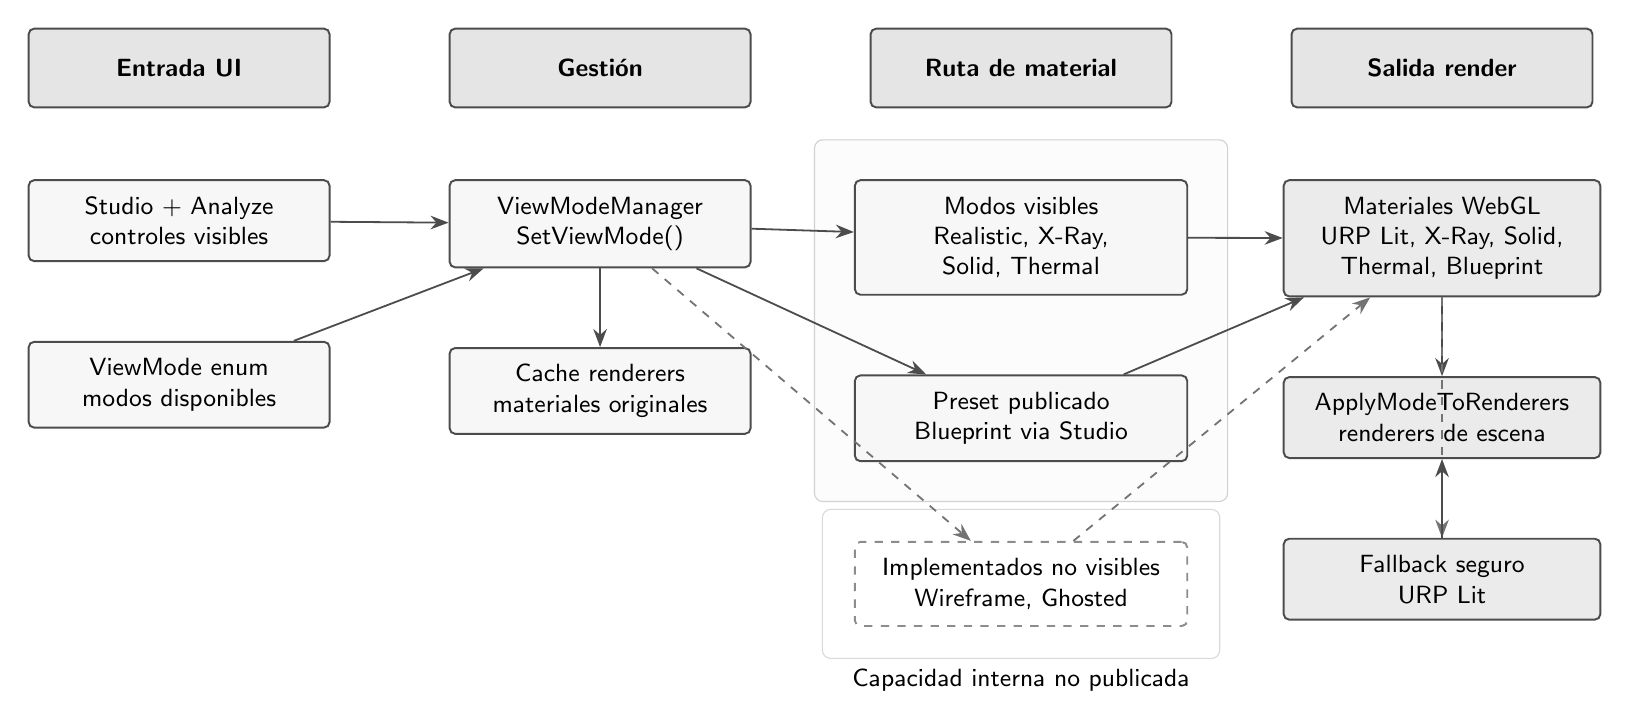
\begin{tikzpicture}[
  font=\sffamily\small,
  node distance=10mm and 15mm,
  box/.style={
    draw=black!70,
    rounded corners=2pt,
    line width=0.7pt,
    fill=black!3,
    align=center,
    inner sep=6pt,
    minimum height=10mm
  },
  head/.style={box, fill=black!10, text width=34mm, font=\sffamily\bfseries\small},
  nodebox/.style={box, text width=34mm},
  route/.style={box, text width=38mm},
  output/.style={box, fill=black!8, text width=36mm},
  hidden/.style={box, fill=white, draw=black!45, dashed, text width=38mm},
  arrow/.style={-{Stealth[length=2.3mm]}, line width=0.65pt, draw=black!70},
  dashedarrow/.style={-{Stealth[length=2.3mm]}, line width=0.65pt, draw=black!55, dashed}
]

\node[head] (uih) {Entrada UI};
\node[head, right=of uih] (managerh) {Gesti\'on};
\node[head, right=of managerh] (routeh) {Ruta de material};
\node[head, right=of routeh] (outh) {Salida render};

\node[nodebox, below=9mm of uih] (ui) {Studio + Analyze\\controles visibles};
\node[nodebox, below=of ui] (enum) {ViewMode enum\\modos disponibles};

\node[nodebox, below=9mm of managerh] (manager) {ViewModeManager\\SetViewMode()};
\node[nodebox, below=of manager] (cache) {Cache renderers\\materiales originales};

\node[route, below=9mm of routeh] (visible) {Modos visibles\\Realistic, X-Ray, Solid, Thermal};
\node[route, below=of visible] (preset) {Preset publicado\\Blueprint via Studio};
\node[hidden, below=of preset] (hidden) {Implementados no visibles\\Wireframe, Ghosted};

\node[output, below=9mm of outh] (materials) {Materiales WebGL\\URP Lit, X-Ray, Solid, Thermal, Blueprint};
\node[output, below=of materials] (apply) {ApplyModeToRenderers\\renderers de escena};
\node[output, below=of apply] (fallback) {Fallback seguro\\URP Lit};

\draw[arrow] (ui) -- (manager);
\draw[arrow] (enum) -- (manager);
\draw[arrow] (manager) -- (cache);
\draw[arrow] (manager) -- (visible);
\draw[arrow] (manager) -- (preset);
\draw[dashedarrow] (manager) -- (hidden);

\draw[arrow] (visible) -- (materials);
\draw[arrow] (preset) -- (materials);
\draw[dashedarrow] (hidden) -- (materials);
\draw[arrow] (materials) -- (apply);
\draw[dashedarrow] (materials) -- (fallback);
\draw[arrow] (fallback) -- (apply);

\begin{scope}[on background layer]
  \node[draw=black!18, rounded corners=3pt, fill=black!1, fit=(visible)(preset), inner sep=5mm, label={[font=\sffamily\small]below:Publicado en el flujo final}] {};
  \node[draw=black!15, rounded corners=3pt, fill=white, fit=(hidden), inner sep=4mm, label={[font=\sffamily\small]below:Capacidad interna no publicada}] {};
\end{scope}

\end{tikzpicture}
\end{document}
